\documentclass[a4paper,12pt]{report}

% Packages
\usepackage[utf8]{inputenc}  % Encoding
\usepackage{amsmath}         % Math symbols
\usepackage{amssymb} % For additional math symbols
\usepackage{graphicx}        % Images
\usepackage[hidelinks]{hyperref}
\usepackage{caption}         % Captions
\usepackage{geometry}        % Page layout
\geometry{a4paper, margin=0.8in}
\usepackage{setspace}        % Line spacing
\usepackage{titlesec}        % Title customization
\usepackage{graphicx}
\usepackage{float}


% Customization
\setcounter{secnumdepth}{3}  % Section numbering depth
\setcounter{tocdepth}{3}     % Table of contents depth
\setlength{\parindent}{0pt}
\renewcommand{\baselinestretch}{1.5}  % Line spacing


% Document starts
\begin{document}

% Title Page
\begin{titlepage}
    \centering

    {\Huge \textbf{Fuzzy Logic and its Applications}}\\[0.5cm]
    {\Large \textit{ Seminar Report}}\\[1.5cm]

    
\includegraphics[width=0.4\textwidth]{nitkkr.png}\\[1cm] % Replace nitkkr.png with the actual path to your logo file.

    \textbf{\Large National Institute of Technology, Kurukshetra}\\[1cm]
    
    \begin{minipage}[t]{0.45\textwidth}
        \raggedright
        \textbf{\large Submitted By:}\\
        {\Large \textbf{Armaan Dhillon}}\\
        {\large Roll No: 12114058}\\
        {\large Department of Electrical Engineering}\\
    \end{minipage}
    \hfill
    \begin{minipage}[t]{0.45\textwidth}
        \raggedleft
        \textbf{\large Submitted To:}\\
        {\Large \textbf{Dr. Jyoti Ohri}}\\
        {\large Department of Electrical Engineering}\\
    \end{minipage}

    \vfill

    {\large January 2025}
\end{titlepage}



% Abstract
\begin{abstract}
    Fuzzy logic has evolved as an effective technique for dealing with complicated, uncertain, and imprecise systems across a wide range of areas. This examination delves into its applications, which range from intelligent control systems and pattern recognition to decision-making and diagnostics. Special emphasis is placed on developments in membership functions (MFs), such as triangular, trapezoidal, Gaussian, and sigmoidal MFs, which serve as the foundation for fuzzy modeling. Recent advances highlight the incorporation of computational techniques such as neural networks and evolutionary algorithms, as well as applications in data analysis, uncertainty management, and intelligent systems. The study also analyzes future directions, focusing on the integration of fuzzy logic with modern technologies such as artificial intelligence and big data analytics. With improved computational powers and expanded applicability, fuzzy logic continues to emerge as a transformational strategy for tackling real-world problems.
\end{abstract}

% Table of Contents
\tableofcontents
\newpage

% Introduction
\chapter{Introduction}
Fuzzy logic, introduced by Lotfi A. Zadeh in 1965, is a mathematical framework designed to model uncertainty and vagueness by moving beyond the rigid boundaries of classical Boolean logic \cite{zadeh1965fuzzy}. Unlike traditional logic, which classifies statements strictly as true or false, fuzzy logic allows intermediate values to represent degrees of truth. This flexibility enables the modeling of complex, real-world situations where imprecision and ambiguity are inherent, such as "slightly hot" or "somewhat large."

The foundation of fuzzy logic lies in fuzzy set theory, where membership grades range between 0 and 1, representing the degree to which an element belongs to a set. Membership functions, which map inputs to these grades, are crucial for translating linguistic variables into a quantitative framework .

Fuzzy logic is particularly useful in applications involving decision-making, control systems, and artificial intelligence, where precise data is often unavailable or impractical. For instance, in industrial automation, fuzzy logic effectively manages noisy sensor data and adjusts control parameters dynamically .

This report provides an overview of fuzzy logic concepts, including fuzzy sets, membership functions, and If-Then rules, emphasizing their role in addressing uncertainty and improving decision-making in complex systems.


% Background
\chapter{Basics of Fuzzy Logic}
\section{Fuzzy Set}

A \textit{fuzzy set} is a mathematical construct designed to address uncertainty and imprecision by allowing an element to belong to a set with varying degrees of membership. Unlike classical sets, which have strict boundaries (either an element is in the set or not), fuzzy sets introduce the concept of partial membership. An element \(x\) in a universal set \(X\) has a membership grade \( \mu_A(x) \in [0, 1] \), where \( \mu_A(x) = 0 \) represents no membership, and \( \mu_A(x) = 1 \) indicates full membership \cite{zadeh1965fuzzy}. Fuzzy sets are particularly effective in systems with linguistic variables, such as ``hot,'' ``cold,'' or ``medium,'' where sharp transitions are unrealistic.

\section{Membership Function}

The \textit{membership function} is a core component of fuzzy sets, defining how the degree of membership is assigned to each element in a fuzzy set. It maps each input value from the universal set \(X\) to a membership value in the interval \([0, 1]\) . Various shapes of membership functions are used, depending on the application:

\begin{figure}[H]
    \centering
    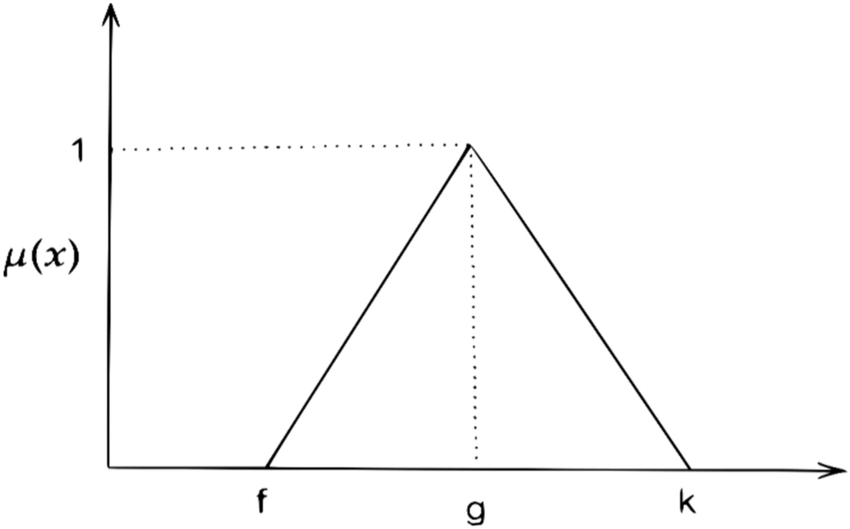
\includegraphics[width=0.6\textwidth]{tmf.png}
    \caption{Triangular Membership Function.}
    \label{fig:triangular}
\end{figure}

\noindent \textbf{Triangular MF}: Defined by three parameters, it provides a simple and computationally efficient representation. This makes it ideal for systems where computational simplicity is paramount.

\begin{figure}[H]
    \centering
    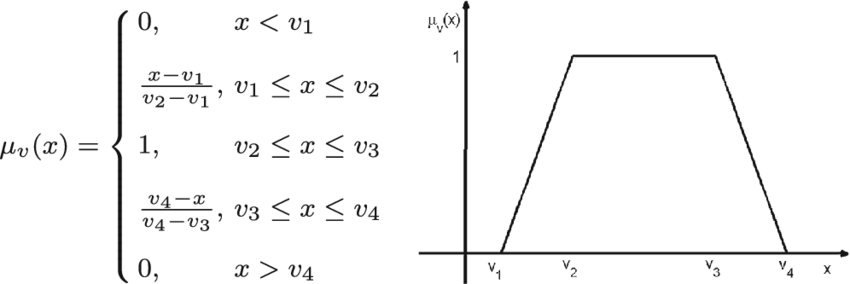
\includegraphics[width=0.6\textwidth]{trapmf.png}
    \caption{Trapezoidal Membership Function.}
    \label{fig:trapezoidal}
\end{figure}

\noindent \textbf{Trapezoidal MF}: Extending the triangular MF, it allows a plateau, making it suitable for broader or less precise categories.

\begin{figure}[H]
    \centering
    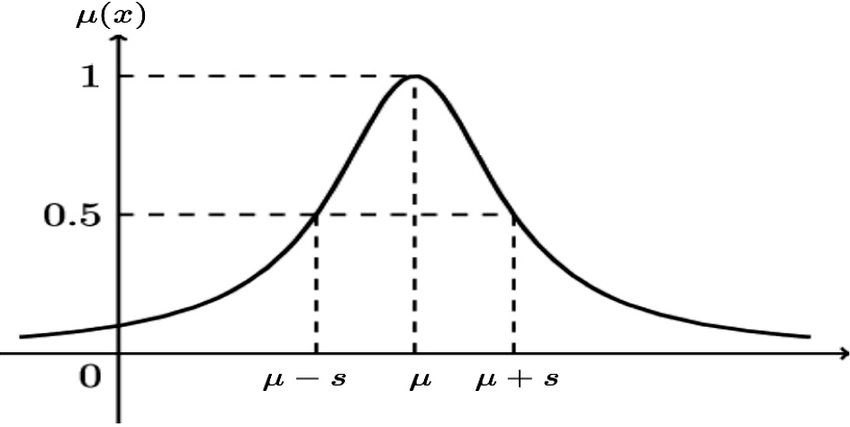
\includegraphics[width=0.6\textwidth]{gaussmf.png}
    \caption{Gaussian Membership Function.}
    \label{fig:gaussian}
\end{figure}

\noindent \textbf{Gaussian MF}: Characterized by its smooth transitions, the Gaussian MF is often employed in applications that require high precision, such as control systems.

\begin{figure}[H]
    \centering
    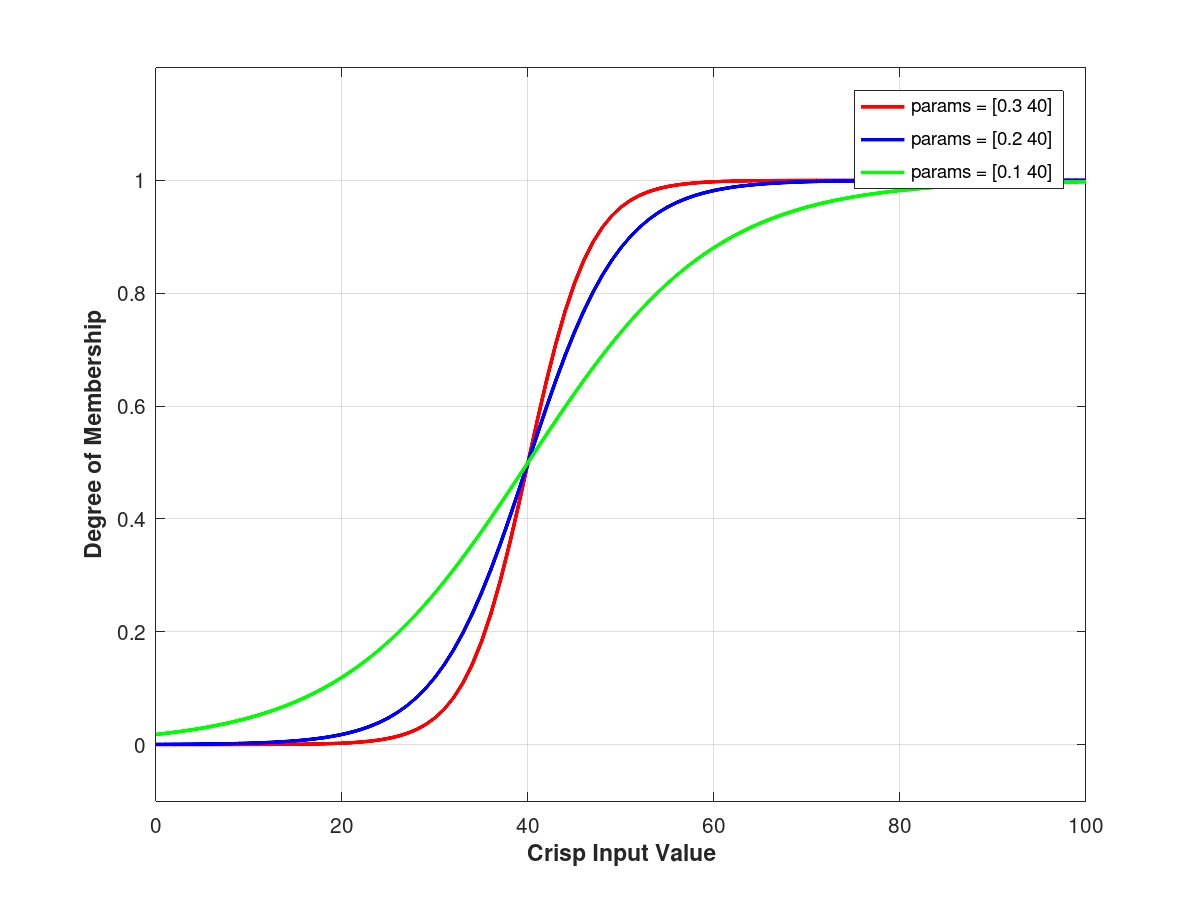
\includegraphics[width=0.6\textwidth]{sigmf.png}
    \caption{Sigmoidal Membership Function.}
    \label{fig:sigmoidal}
\end{figure}

\noindent \textbf{Sigmoidal MF}: Useful for asymmetrical membership distributions, it is particularly effective in scenarios requiring gradual increases or decreases in membership.


The choice of membership function depends on the problem's requirements and the level of computational complexity acceptable.

\section{If-Then Rule Structure}

Fuzzy logic uses a system of \textit{If-Then rules} to model decision-making processes. These rules are the building blocks of a fuzzy inference system (FIS). Each rule consists of:  

\begin{itemize}
    \item \textbf{Antecedent (If part)}: Conditions represented by fuzzy sets.
    \item \textbf{Consequent (Then part)}: Actions or outputs triggered when conditions are met.
\end{itemize}

For example:  
\textbf{IF} temperature is high \textbf{AND} humidity is low \textbf{THEN} increase fan speed.

Rules operate using fuzzy logic operators:  
\begin{itemize}
    \item AND: Takes the minimum membership value between conditions.
    \item OR: Takes the maximum membership value.
    \item NOT: Complements the membership value.
\end{itemize}

These rules are aggregated and processed in the inference system to produce a fuzzy output .

\section{Basic Fuzzy Control System Structure}

The figure below illustrates the basic structure of a fuzzy control system, which consists of three primary components: \textbf{Fuzzification}, \textbf{Fuzzy Inference}, and \textbf{Defuzzification}, with a \textbf{Fuzzy Rule Base} integrated into the inference process.

\begin{figure}[h]
    \centering
    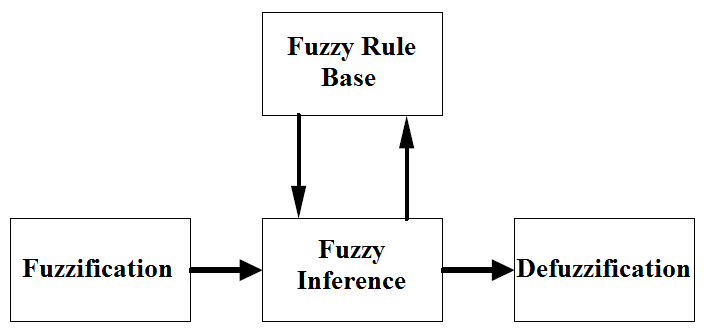
\includegraphics[width=0.6\textwidth]{image.png}
    \caption{Basic fuzzy control system structure.}
\end{figure}

\subsection*{1. Fuzzification}
This is the process of converting crisp input values (real-world measurements) into fuzzy sets. Input data is mapped to corresponding degrees of membership within predefined fuzzy sets using membership functions.

\subsection*{2. Fuzzy Rule Base}
This component contains a collection of linguistic rules defined by experts or derived from system knowledge. These rules relate the fuzzy input variables to the desired output variables using \textit{IF-THEN} statements. For example, a rule might state: 
\begin{quote}
    \textit{IF the liquid level is high, THEN reduce the inflow.}
\end{quote}

\subsection*{3. Fuzzy Inference}
In this stage, the fuzzy inputs are processed according to the rules in the rule base to generate fuzzy output sets. A combination of fuzzy logic operations (e.g., AND, OR) and membership functions is used to determine the resulting fuzzy output.

\subsection*{4. Defuzzification}
The fuzzy output generated by the inference engine is converted back into a crisp value (a real-world actionable output). This is achieved using defuzzification methods such as the centroid, maximum, or average method.

\textbf{Purpose:} The fuzzy control system enables handling of imprecise or uncertain data by using linguistic variables and rule-based reasoning. It is particularly useful for systems where mathematical modeling is complex or impossible.

Fuzzy logic is widely applied in control systems, expert systems, and pattern recognition, where conventional binary logic struggles to capture real-world ambiguities.



% Applications
\chapter{Applications of Fuzzy Logic}

\section{Medical Sciences}
Fuzzy logic has emerged as a valuable tool in medical sciences, aiding in the management of uncertainty in diagnosis, therapy, and patient monitoring. It helps to evaluate complex medical data and integrate Western and Eastern medicine for comprehensive care. Systems such as "DoctorMoon" use fuzzy rules to deal with ambiguous symptoms, allowing for reliable diagnosis of a variety of ailments. In traditional Oriental medicine, fuzzy logic formalizes ambiguous expressions like "severe pain," which improves therapies such as acupuncture. Furthermore, it supports in real-time monitoring by simulating medical notions such as "high fever," allowing for timely and precise decisions. Overall, fuzzy logic improves dependability and precision in healthcare. \cite{phuong2001fuzzy}

\section{Control Systems}
Fuzzy logic control has gained significant attention in recent decades for its ability to handle uncertainty and imprecision in control systems \cite{nazemizadeh2014application}. This approach utilizes linguistic variables and fuzzy sets to model system behavior, offering advantages in implementing control laws based on knowledge or linguistic descriptions. Fuzzy logic controllers have been successfully applied in various fields, from automatic train operation to flight systems \cite{langari1999past}. The semantic transparency of fuzzy logic enables efficient development of control strategies for systems with low-order dynamics and weak nonlinearities \cite{langari1999past}. Furthermore, fuzzy control systems analyze input data using continuous values in the [0, 1] interval, allowing for the expression of solutions in natural language \cite{voskoglou2019methods}. This feature facilitates the mechanization of tasks previously performed by humans. Applications of fuzzy logic control include robotics \cite{nazemizadeh2014application}, temperature control , and building heating systems \cite{voskoglou2019methods}.
\section{Decision Support Systems}
Fuzzy logic (FL) has emerged as a valuable tool in Decision Support Systems (DSS) for handling uncertainty and imprecision in decision-making processes. FL enables DSS to manage ambiguous inputs and provide precise solutions, mimicking human reasoning . Its applications span various sectors, offering practical benefits and maturity in implementation \cite{metaxiotis2004new}. FL-based DSS can effectively analyze enterprise conditions, supporting decision-makers in risk environments and potentially preventing bankruptcy \cite{tishkina2018application}. While Type-1 Fuzzy Sets are commonly used, Type-2 Fuzzy Sets can better represent uncertainties, especially when dealing with multiple expert opinions \cite{comas2014type}. FL facilitates the explanation of decision outcomes through explicit knowledge representation, enhancing system readability . As DSS continue to evolve, FL integration promises to improve their ability to handle complex, real-world decision scenarios with vague and uncertain data.

% Advantages and Challenges
\chapter{Advantages and Challenges}
\section{Advantages}
Fuzzy logic controllers provide considerable benefits, especially in systems with complex, nonlinear, or poorly characterized dynamics. They do not rely on a precise mathematical model, making them more versatile and easier to employ in real-world circumstances where system characteristics can change. Furthermore, fuzzy logic uses expert-defined rules to simulate human decision-making, allowing it to successfully deal with uncertainty and operational changes. These controllers are noted for their faster response times, increased stability, and higher precision when compared to traditional PID controllers, making them the preferred choice in applications that require high performance and adaptability \cite{diouf2021comparative}.
Fuzzy logic controllers effectively manage uncertainty and nonlinear dynamics, providing precise and adaptive control without the need for a formal mathematical model. They promote scalability by allowing for additional rules and smooth modifications near target ranges, making them excellent for quick and adaptable applications\cite{ashbaughadvantages}.
\section{Challenges}
Fuzzy logic controllers also have some drawbacks. One significant limitation is the lack of established design rules, which might complicate implementation. The success of these controllers is strongly reliant on the quality of the rule base, which necessitates extensive input from domain experts to assure peak performance. Furthermore, the design and tuning processes for fuzzy logic systems are frequently more involved than those for PID controllers. Despite these obstacles, fuzzy logic is a useful tool for controlling complex and dynamic systems\cite{diouf2021comparative}.
Fuzzy logic controller design is complex and time-consuming, necessitating precise parameter and rule adjustment. Their performance is largely dependent on configuration, and simpler controllers may produce comparable results with substantially less work\cite{ashbaughadvantages}.

% Trends and Future Directions
\chapter{Trends and Future Directions}
Fuzzy logic continues to evolve and find applications across diverse industries, demonstrating its expanding utility in tackling complex problems. Recent advancements include the development of type-2 fuzzy systems that are particularly effective in handling uncertainties, making them suitable for tasks such as intelligent control and pattern recognition \cite{mittal2020comprehensive}. The field is also witnessing a shift towards second-generation systems, which integrate fuzzy logic with computational techniques like neural networks and genetic algorithms. These hybrid approaches leverage the strengths of each method, resulting in more robust and adaptive solutions while aligning fuzzy logic design methodologies closer to those of conventional control systems . Future directions for fuzzy logic emphasize its integration with modern technologies such as artificial intelligence, machine learning, and big data analytics, facilitating its application in areas beyond control, including data analysis, diagnosis, and decision support systems \cite{chalamalasetty2024envisioning}. Researchers continue to emphasize the need for consolidating existing results to strengthen the foundation of the field while simultaneously exploring innovative paths. This dual focus is expected to lead to interesting developments in uncertainty management and intelligent systems \cite{tabacchi2015future}. As computational capabilities improve, fuzzy logic systems are poised to address increasingly complex real-world scenarios, potentially driving revolutionary advancements in intelligent technologies \cite{chalamalasetty2024envisioning}.

% Conclusion
\chapter{Conclusion}
Fuzzy logic has demonstrated its adaptability and effectiveness in handling a variety of applications, especially in settings that are marked by imprecision and uncertainty. As evidenced by the employment of different membership functions, its primary strength is its capacity to approximate reasoning and represent linguistic factors. Fuzzy logic has become a key component of intelligent systems due to the development of hybrid systems that integrate it with neural networks, evolutionary algorithms, and other cutting-edge computing methods. Its place in contemporary technology has also been cemented by developments and their uses in data-driven diagnostics and decision-making.The field is set to reach even higher heights as computing power keeps increasing, expanding its influence to domains like autonomous systems, big data, and artificial intelligence. In order to handle new issues and spur innovation in intelligent technologies, this review emphasizes the necessity of further investigation and integration of fuzzy logic approaches.

% References
\renewcommand{\bibname}{References}

\bibliographystyle{IEEEtran}
\bibliography{references}

% End of document
\end{document}
